% \documentclass[12pt]{article}
% \usepackage{graphicx}
% \usepackage{epstopdf}
% \usepackage[spanish]{babel}
% \selectlanguage{spanish}
% \usepackage[utf8]{inputenc}
% \usepackage{hyperref}
% \usepackage[left=3cm,top=3cm,right=3cm,bottom= 2.5cm,nohead,nofoot]{geometry}
% \usepackage{braket}
% \usepackage{datenumber}
% \usepackage{textcomp}
% \usepackage{chemfig}%figuras Quimica
% \usepackage[version=4]{mhchem}%nombres compuestos quimicos
% %\newdate{date}{10}{05}{2013}
% \begin{document}
% \begin{figure}%[h]

% \end{figure}

\begin{center}
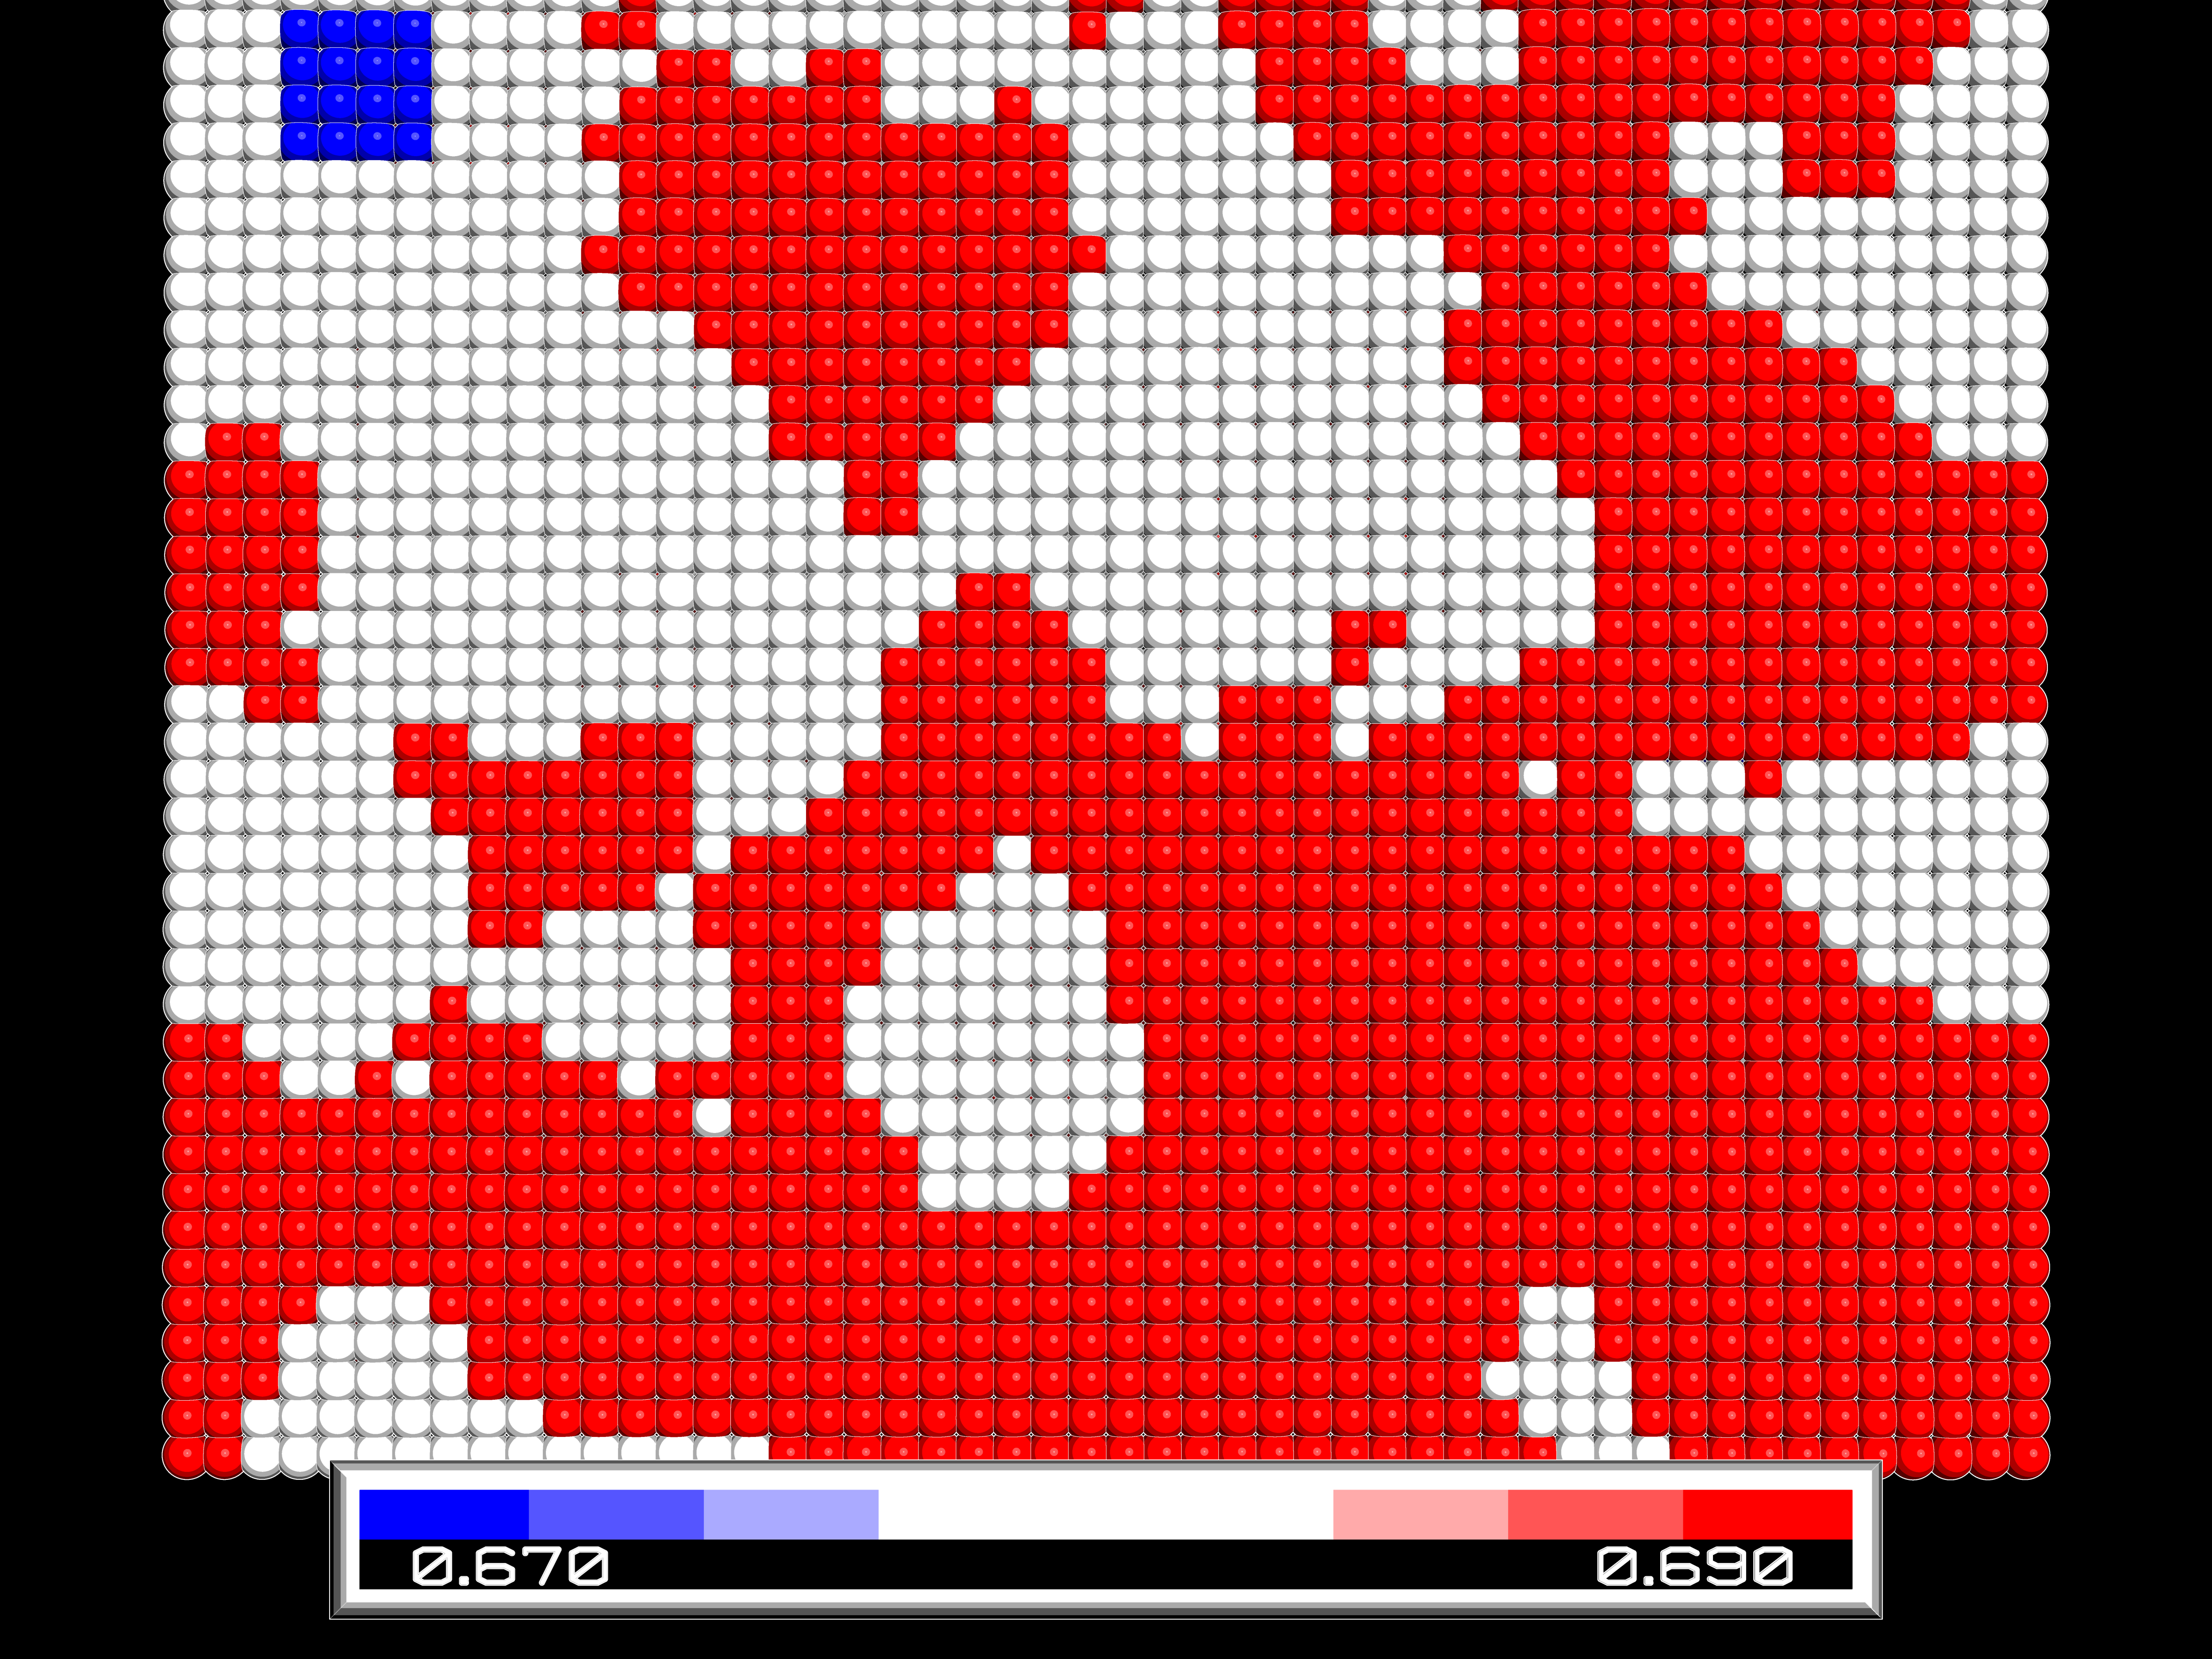
\includegraphics[scale=0.01]{Plots/glomepro/snap_MEM-DMPG_1_do.png}
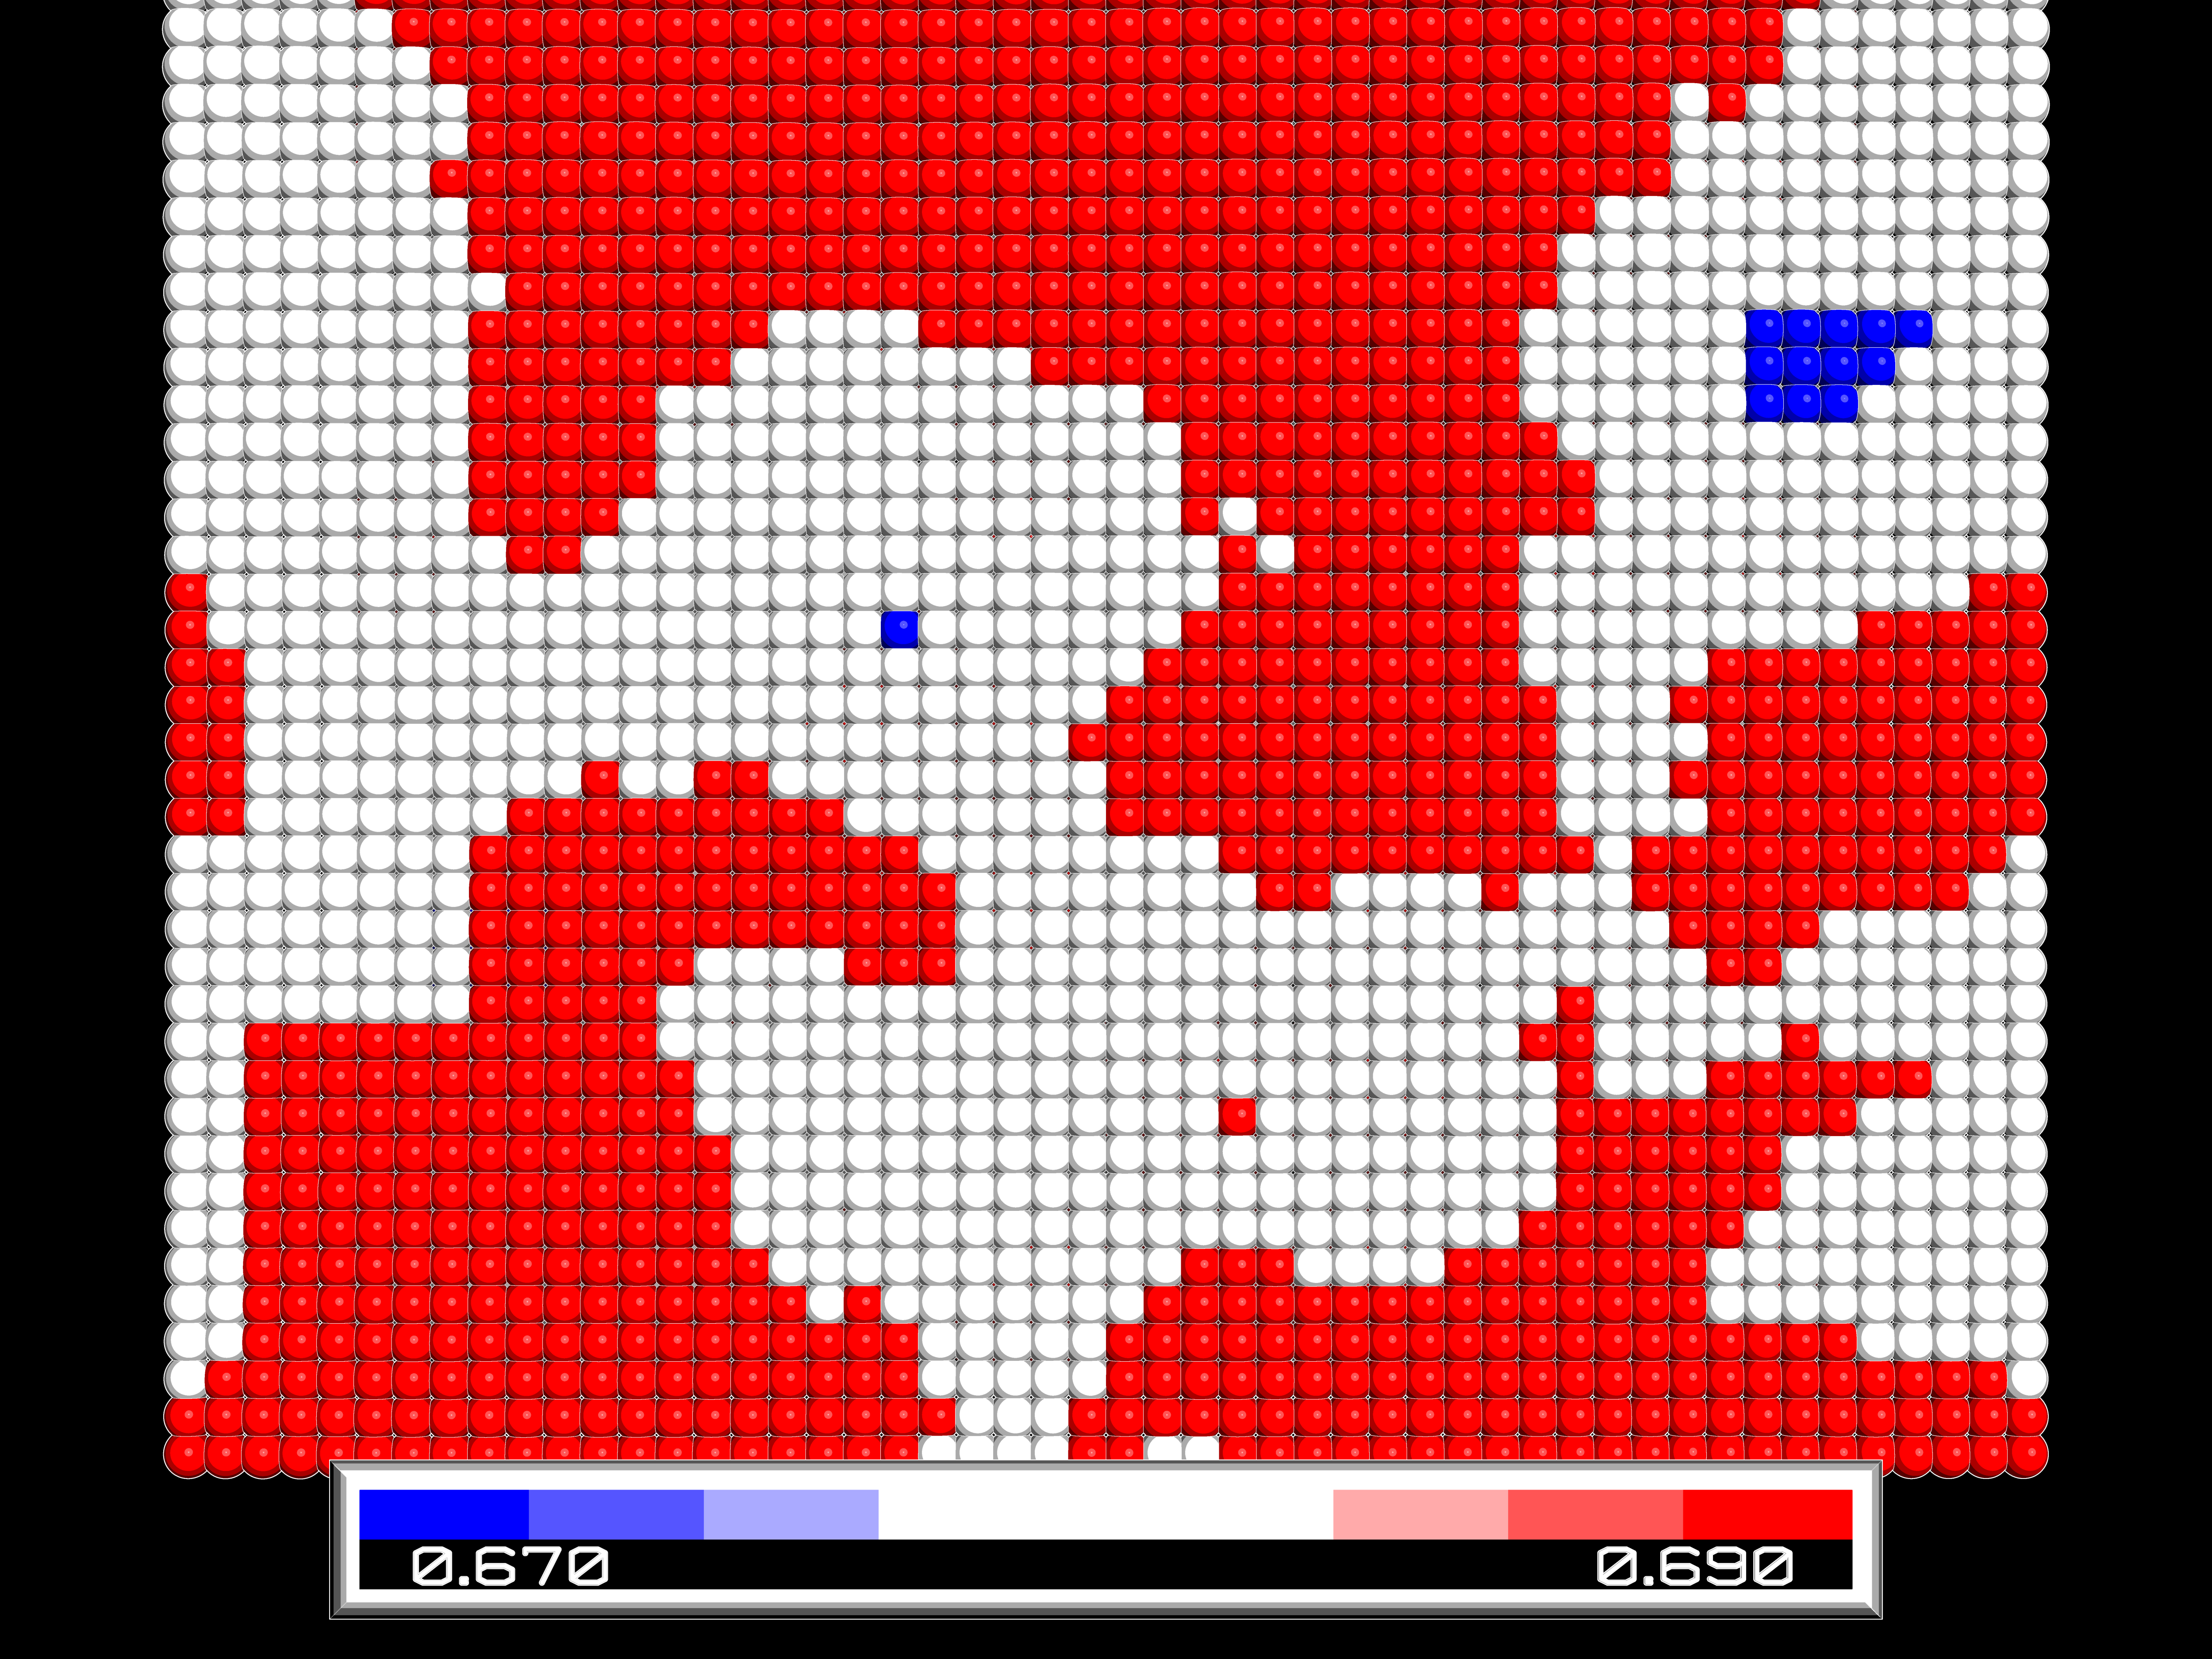
\includegraphics[scale=0.01]{Plots/glomepro/snap_MEM-DMPG_1_up.png}
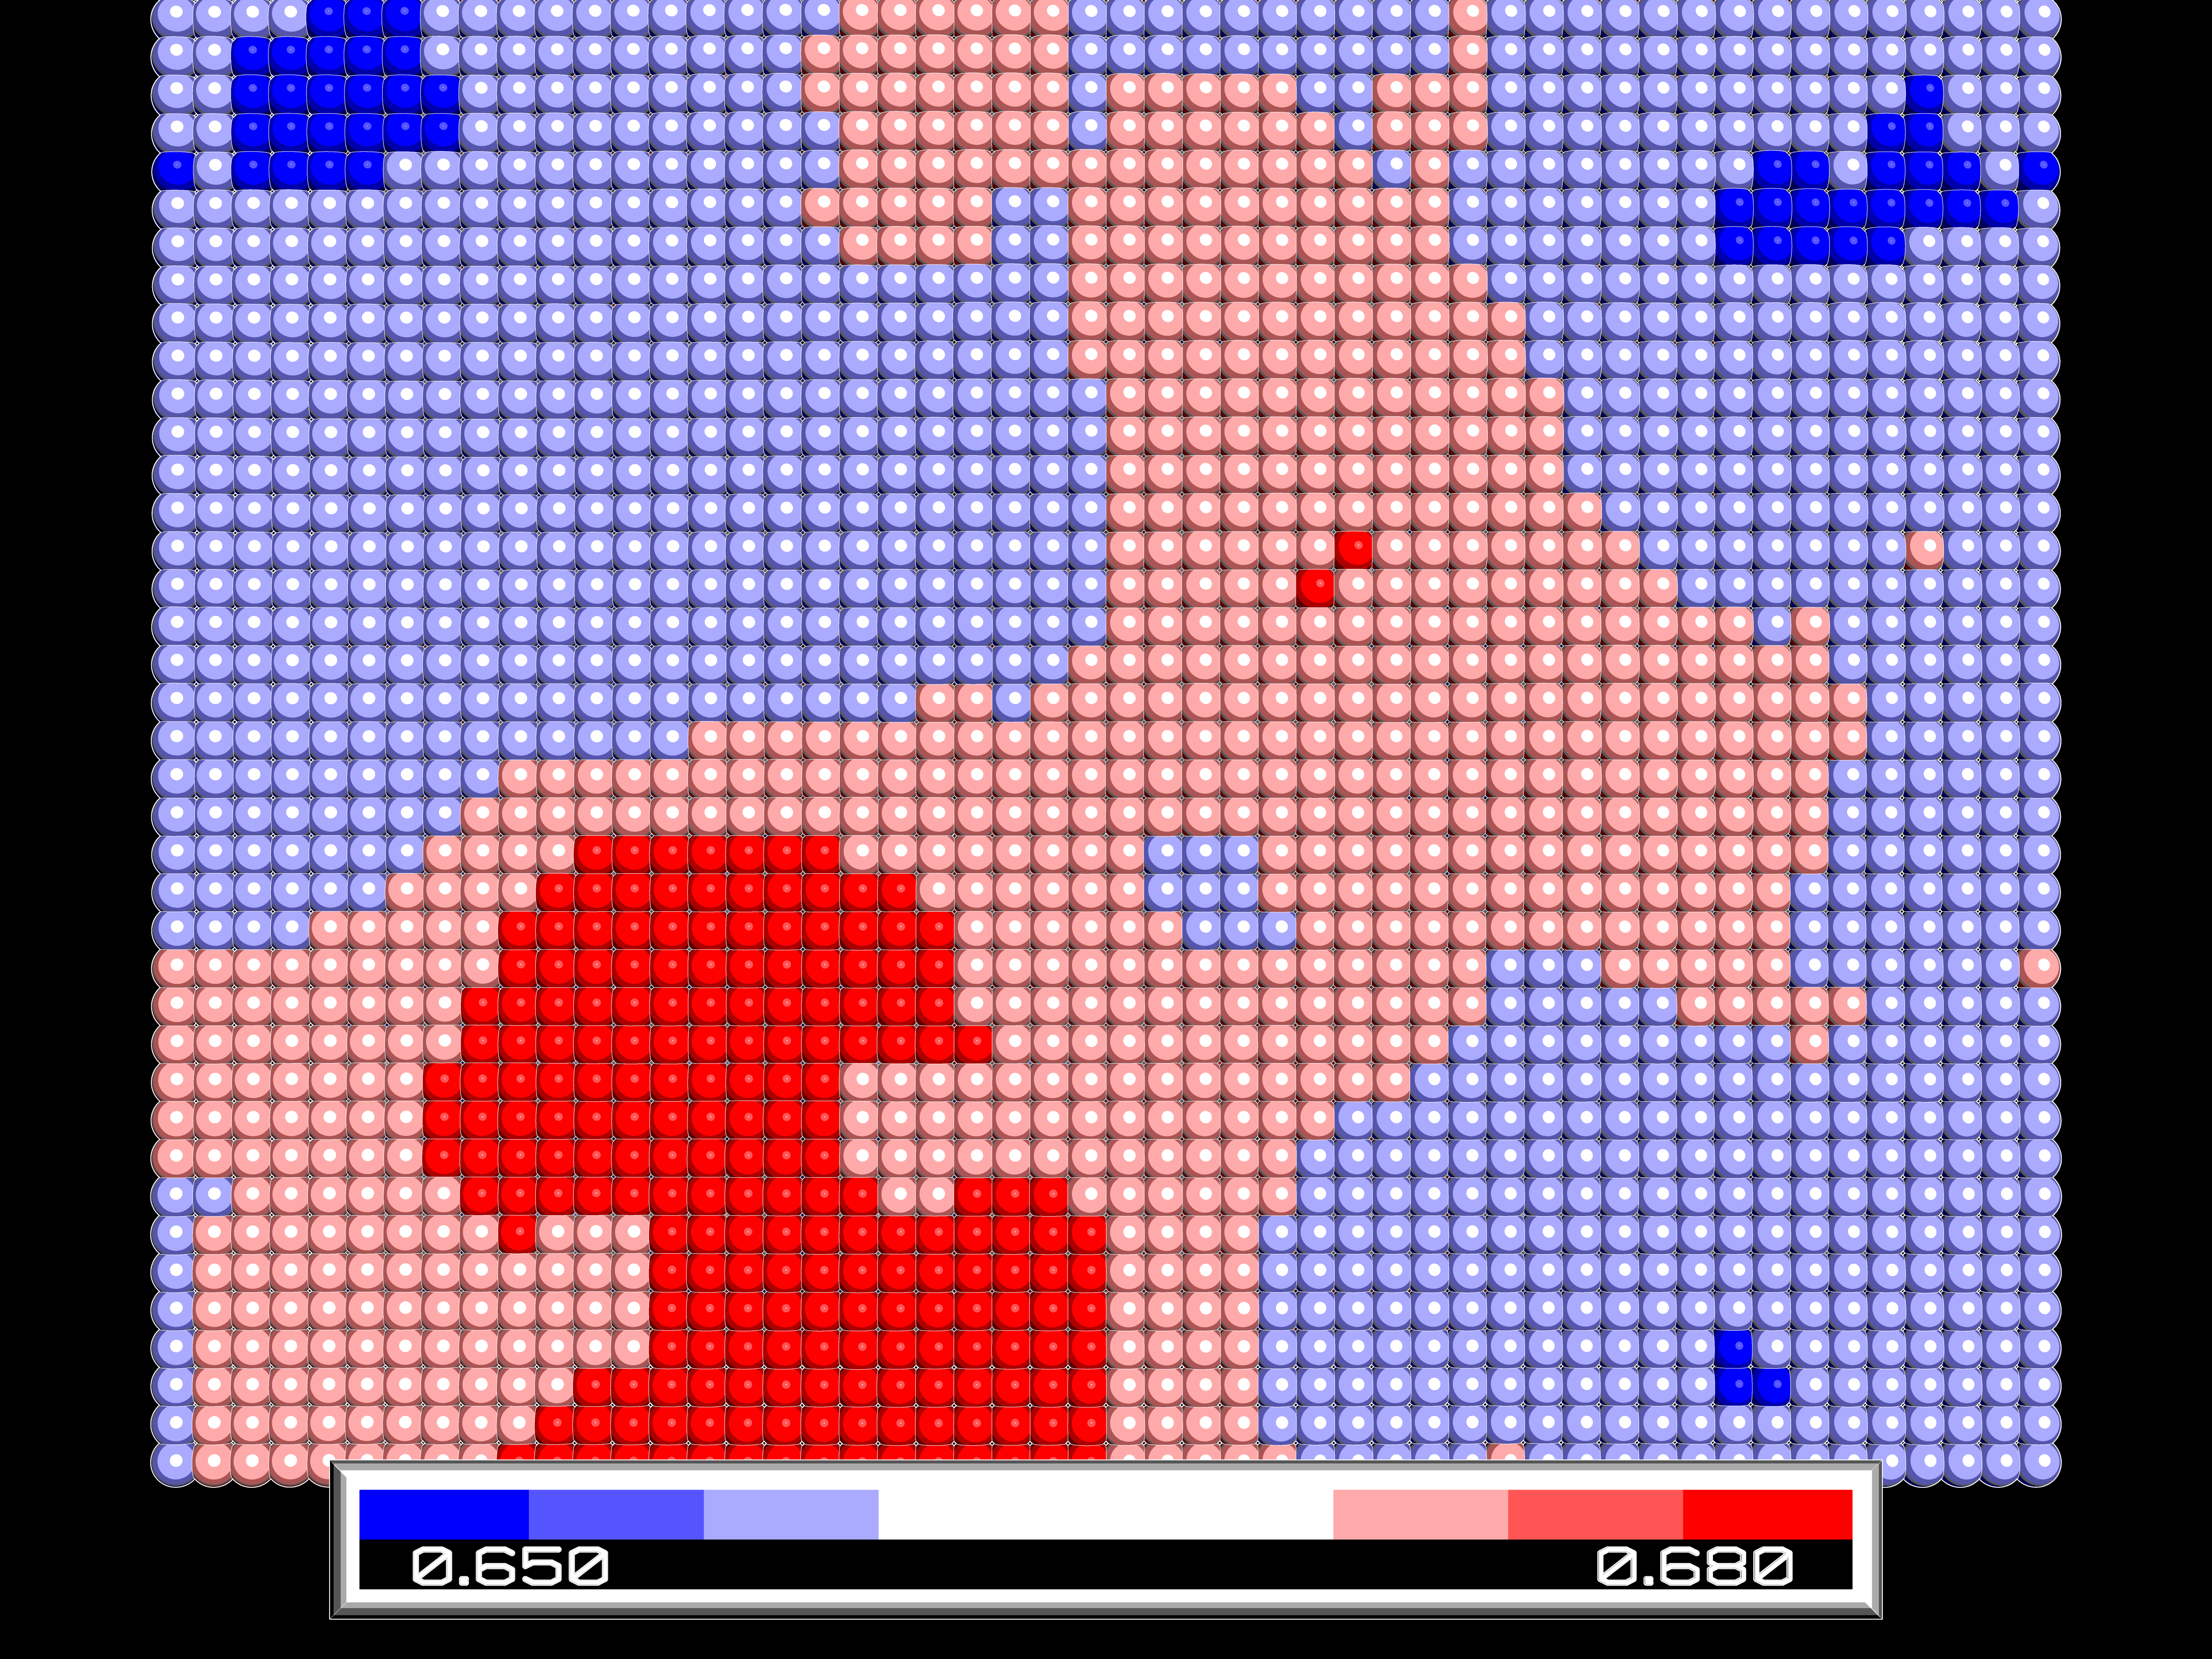
\includegraphics[scale=0.01]{Plots/glomepro/snap_MEM-DPPG_1_do.png}
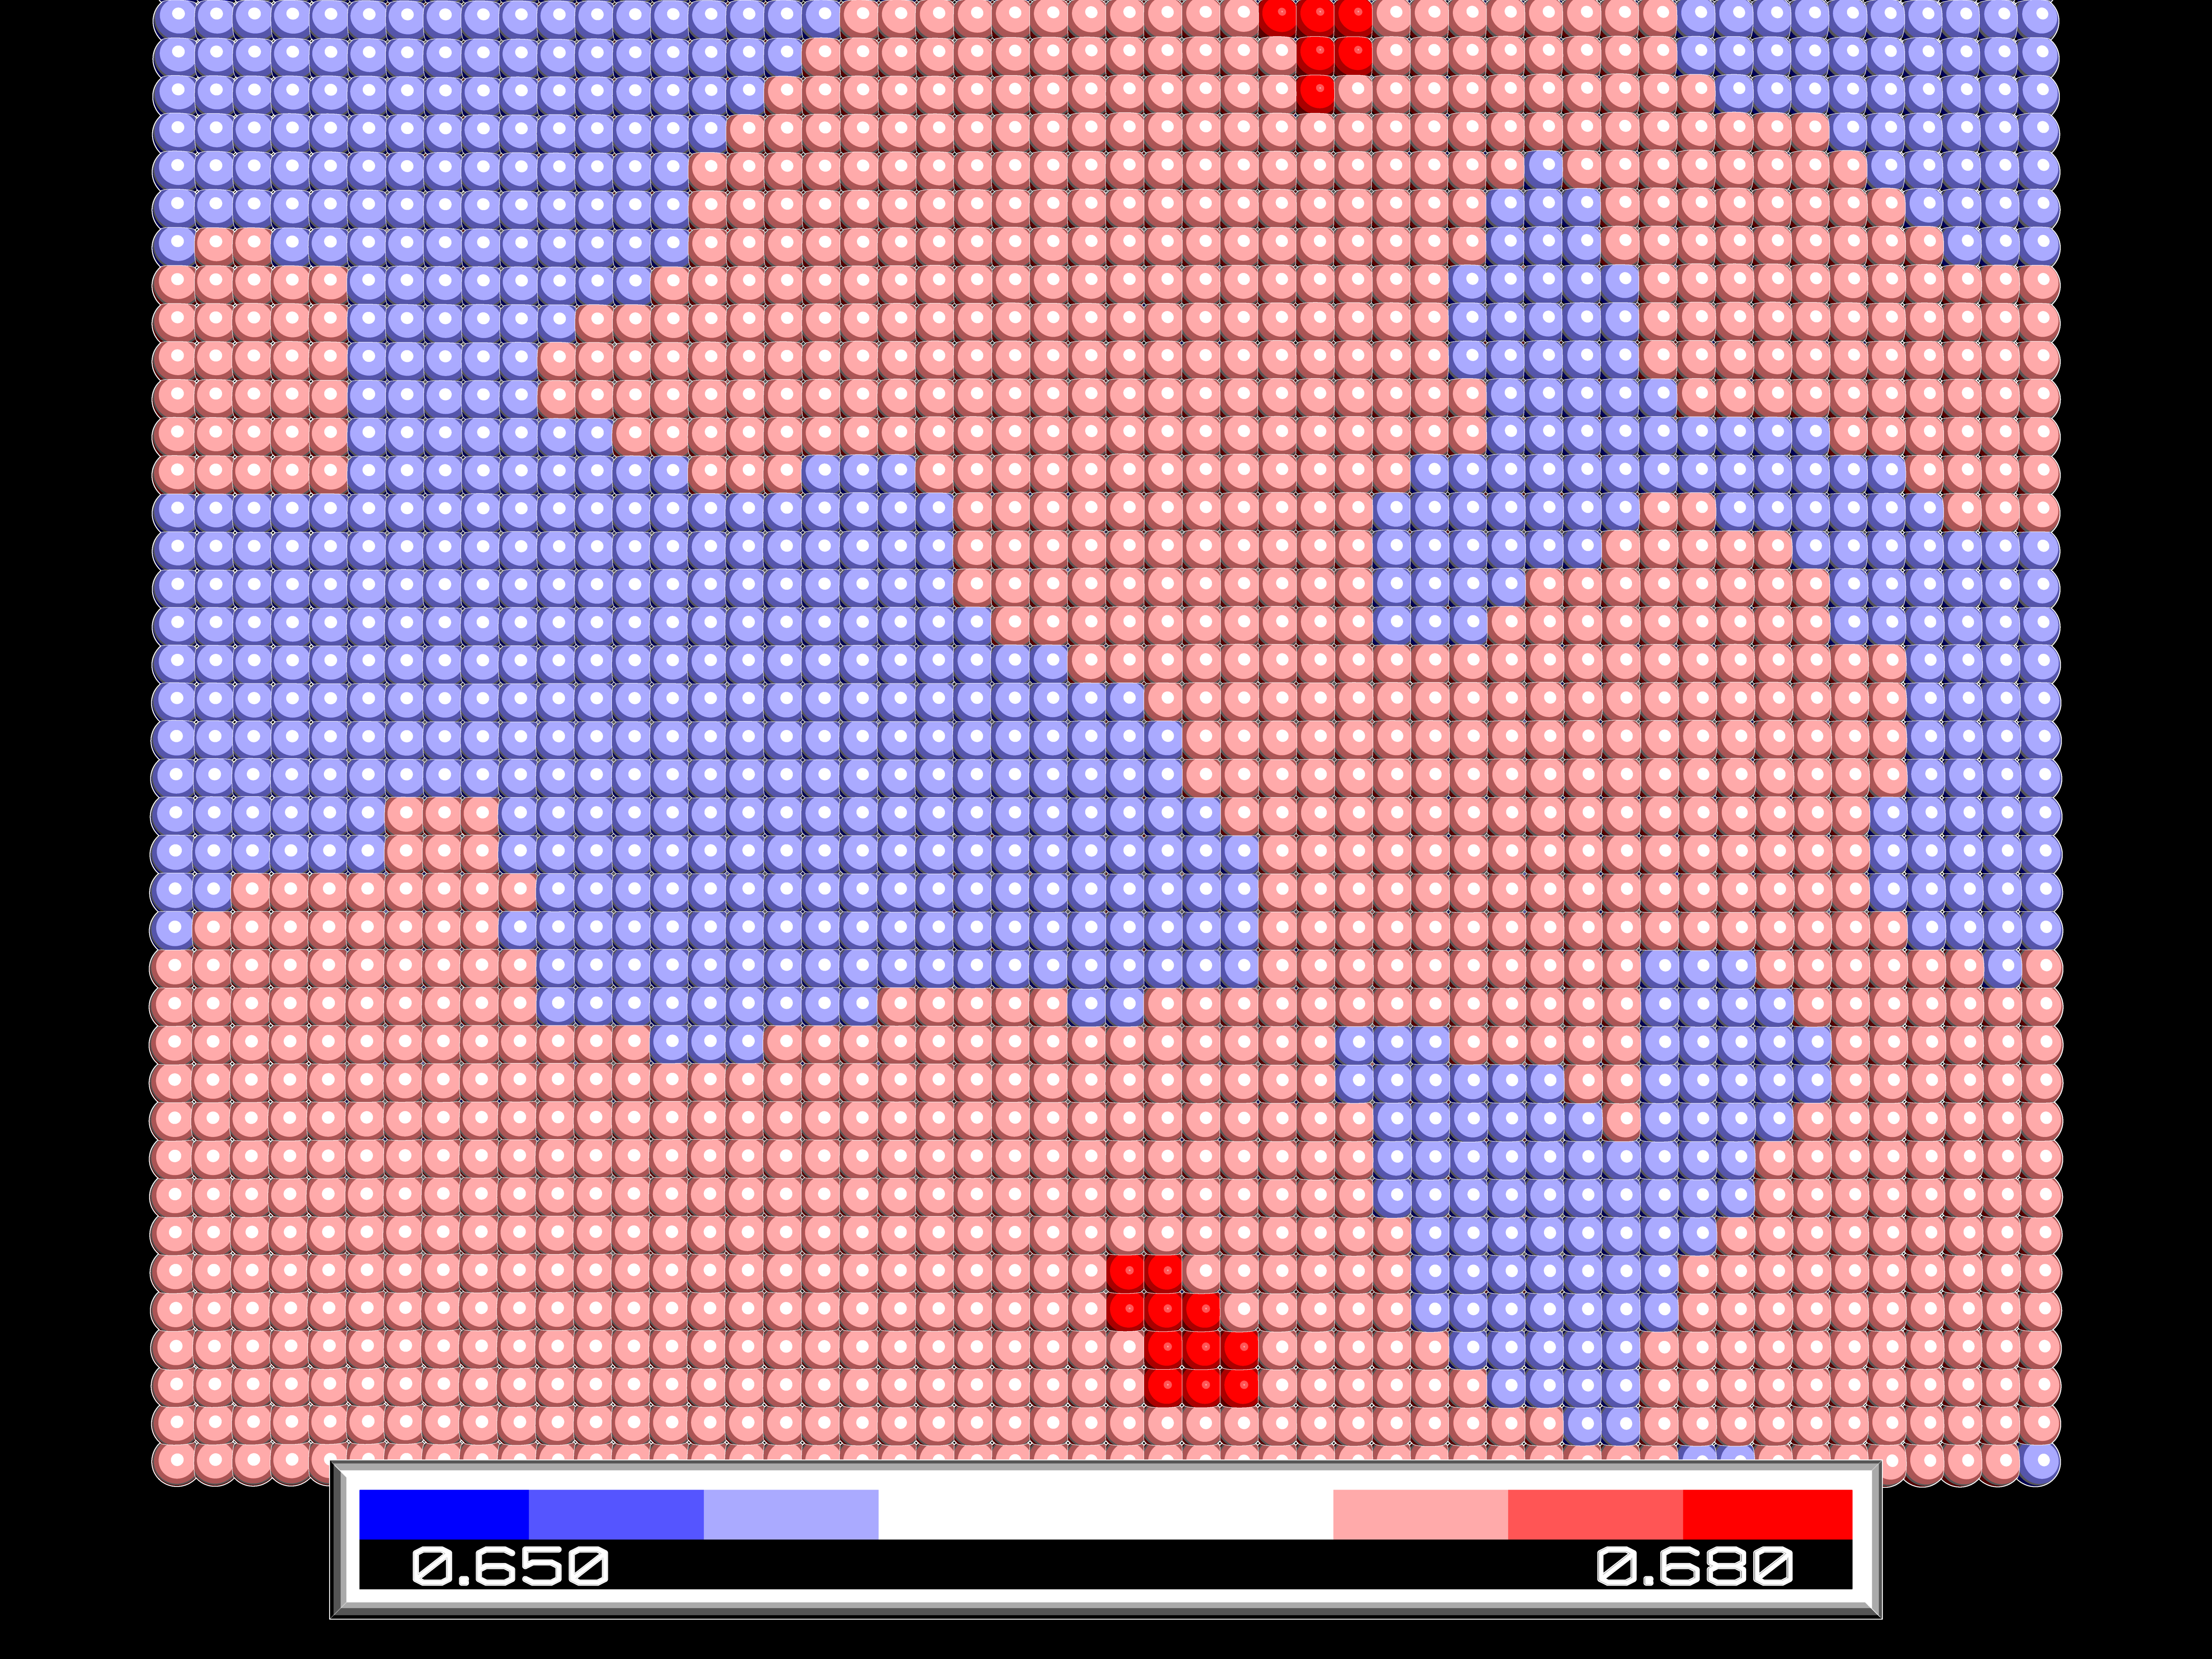
\includegraphics[scale=0.01]{Plots/glomepro/snap_MEM-DPPG_1_up.png}
\end{center} 

%  \end{document}
